\documentclass[tikz,border=12pt]{standalone}
\usepackage[T1]{fontenc}
\usepackage{lmodern,amsmath,amssymb}
\usetikzlibrary{arrows.meta}
\definecolor{ink}{HTML}{183444}
\definecolor{blue}{HTML}{1B6780}
\definecolor{amber}{HTML}{AD601A}
\begin{document}
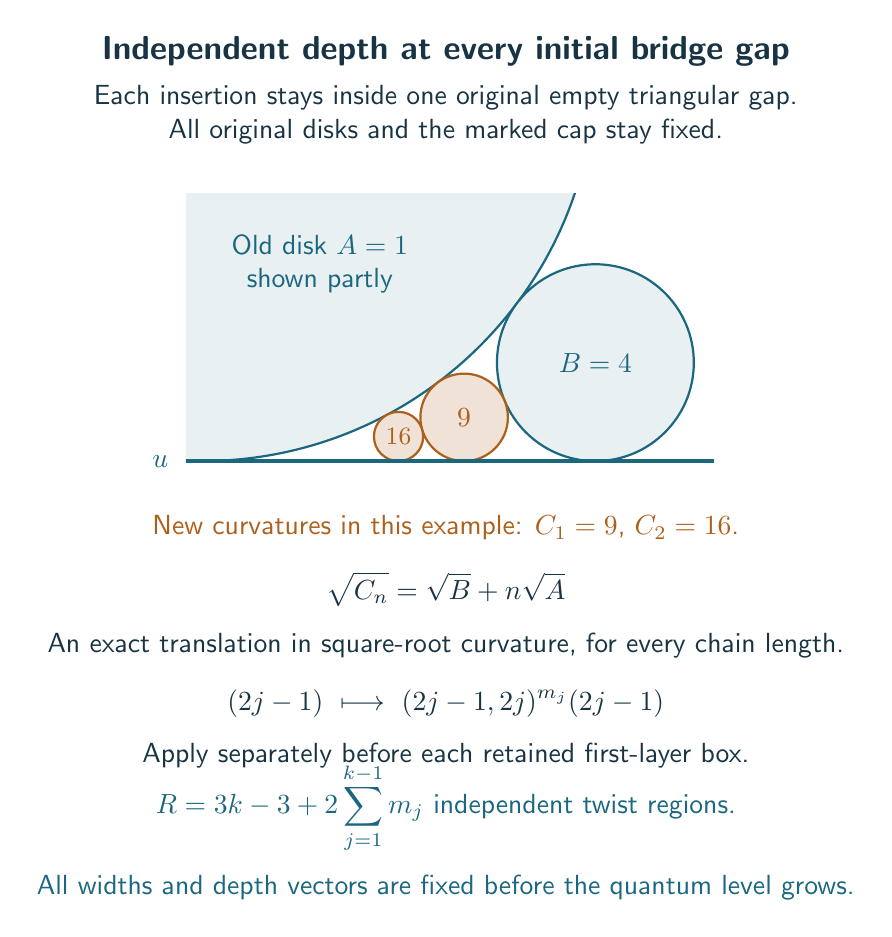
\begin{tikzpicture}[x=5cm,y=5cm,font=\sffamily,text=ink,>=Stealth]
 \node[font=\sffamily\large\bfseries] at (.62,1.04)
 {Independent depth at every initial bridge gap};
 \node[align=center] at (.62,.88)
 {Each insertion stays inside one original empty triangular gap.\\
 All original disks and the marked cap stay fixed.};
 \begin{scope}
  \clip (-.04,0) rectangle (1.3,.68);
  \draw[blue,thick,fill=blue!10] (0,1) circle (1);
  \draw[blue,thick,fill=blue!10] (1,.25) circle (.25);
  \draw[amber,thick,fill=amber!18] ({2/3},{1/9}) circle ({1/9});
  \draw[amber,thick,fill=amber!18] (.5,{1/16}) circle ({1/16});
 \end{scope}
 \draw[blue,very thick] (-.04,0)--(1.3,0);
 \node[anchor=east,text=blue] at (-.06,0) {$u$};
 \node[align=center,text=blue] at (.3,.5) {Old disk $A=1$\\shown partly};
 \node[text=blue] at (1,.25) {$B=4$};
 \node[text=amber] at ({2/3},{1/9}) {$9$};
 \node[font=\sffamily\small,text=amber] at (.5,{1/16}) {$16$};
 \node[align=center,text=amber] at (.62,-.17)
 {New curvatures in this example: $C_1=9$, $C_2=16$.};
 \node[align=center] at (.62,-.39)
 {$\displaystyle \sqrt{C_n}=\sqrt B+n\sqrt A$\\[7pt]
 An exact translation in square-root curvature, for every chain length.};
 \node[align=center] at (.62,-.68)
 {$\displaystyle (2j-1)\ \longmapsto\ (2j-1,2j)^{m_j}(2j-1)$\\[7pt]
 Apply separately before each retained first-layer box.};
 \node[align=center,text=blue] at (.62,-.94)
 {$\displaystyle R=3k-3+2\sum_{j=1}^{k-1}m_j$ independent twist regions.\\[7pt]
 All widths and depth vectors are fixed before the quantum level grows.};
\end{tikzpicture}
\end{document}
